Реестр Windows или системный реестр --- иерархически построенная база данных параметров и настроек в большинстве операционных систем Microsoft Windows. Реестр содержит информацию и настройки для аппаратного обеспечения, программного обеспечения, профилей пользователей, предустановки. Большинство изменений в Панели управления, ассоциации файлов, системные политики, список установленного ПО фиксируются в реестре. И именно поэтому получение его данных является крайне важной задачей для дальнейшего исследования в ходе компьютерной экспертизы. 


Конечной целью работы является разработка программного модуля (winreg) для конвертирования данных из реестра в подходящий для дальнейшего исследования формат. Для достижения данной цели были установлены следующие задачи, разбитые на три этапа.


Этап первый --- <<введение>>:
\begin{itemize}
  \item ознакомление с coex --- системой для комплексного анализа использования операционных систем семейств Microsoft Windows;
  \item ознакомление с открытой средой разработки QtCreator;
  \item ознакомление со системой верстки документов Latex;
  \item ознакомление cо системой контроля версия Git, обучение основные ее возможностям.
\end{itemize}

Этап второй --- <<исследование>>:
\begin{itemize}
  \item исследование модели формирования и структуры реестра Windows;
  \item исследование готовых решений для работы реестром Windows.
\end{itemize}

Этап третий --- <<разработка>>:
\begin{itemize}
  \item выбор метода получение информации из реестра;
  \item разработка приложения.
\end{itemize}

\subsubsection{Этап второй --- <<исследование>>. Структура и модель формирования}
Как и было сказано ранее, реестр Windows --- иерархически построенная база данных, формируемая на основе конфигурации ПК и пользовательских или программных настроек. В собранном виде он имеет древовидный вид с пятью корневыми разделами (табл.~\ref{tab:roots}).

% таблица – Корневые разделы реестра и их краткое описание
\begin{table}[ht]
\caption{Корневые разделы реестра и их краткое описание}
\label{tab:roots}
\begin{center}
\begin{tabular}{|p{8cm}|p{9cm}|}
\hline
HKEY\_CLASSES\_ROOT & Подраздел HKEY\_LOCAL\_MACHINE\textbackslash Software \\
\hline
HKEY\_CURRENT\_USER & Корневой для данных конфигурации пользователя; подраздел HKEY\_USERS \\
\hline
HKEY\_LOCAL\_MACHINE & Параметры конфигурации ПК \\
\hline
HKEY\_USERS & Все активные профили пользователей \\
\hline
HKEY\_CURRENT\_CONFIG & Информации об оборудовании ПК \\
\hline
\end{tabular}
\end{center}
\end{table}

Каждый раздел состоит из некоторого количества подразделов, отвечающих за различные настройки программного обеспечения, самой операционной системы или служебную информацию.


Реестр Windows формируется в момент загрузки операционной системы из некоторых исходных файлов, список которых может быть найден по пути: HKEY\_LOCAL\_MACHINE\textbackslash SYSTEM\textbackslash CurrentControlSet\textbackslash Control\textbackslash hivelist (рис.~\ref{hivelist:hivelist}).

\begin{figure}[ht]                                % сюда рисунок hivelist       
\center{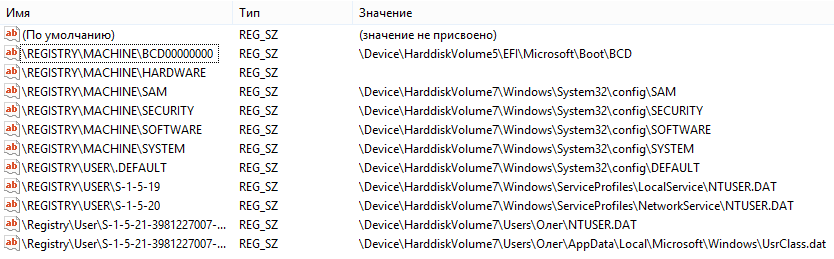
\includegraphics[width=0.8\linewidth]{hivelist}}
\caption{Пример содержимого hivelist}
\label{hivelist:hivelist}
\end{figure}


Непосредственно сам механизм сбора на данном этапе перестал быть интересен, поскольку интерес теперь представляют исходные файлы (далее <<сырые>> файлы реестра).

\subsubsection{Этап второй --- <<исследование>>. Исследование готовых решений}
Поскольку система комплексного анализа использования Windows не предполагает непосредственного запуска самой исследуемой ОС, дальнейшую работу необходимо вести имя лишь доступ к файловой системе, что, в свою очередь, предполагает работу лишь с <<сырыми>> файлами реестра. Для этого необходимо специальное ПО.


Были рассмотрены два приложения для работы с исходными файлами реестра: Fred (Forensic Registry EDitor) и chntpw.


Chntpw --- утилита, позволяющая работать с <<сырыми>> файлами реестра. Изначально она была написана лишь для сбора паролей Windows, но в последствии была расширена для редактирования всего реестра (рис.~\ref{chntpw:chntpw}).

\begin{figure}[ht]                                % сюда рисунок Chntpw     
\center{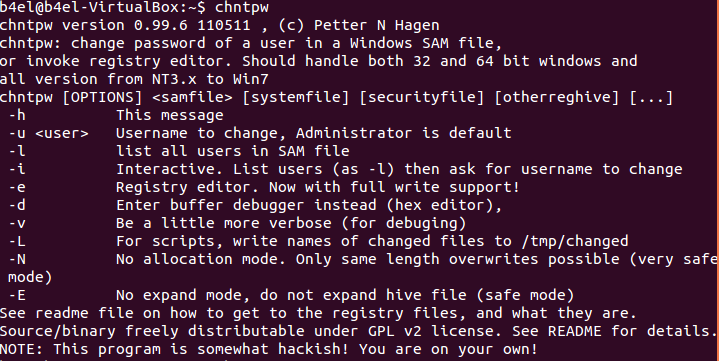
\includegraphics[width=0.8\linewidth]{chntpw}}
\caption{Параметры запуска chntpw}
\label{chntpw:chntpw}
\end{figure}


Плюсы и минусы использования данной утилиты приведены в таблице~\ref{tab:pluses}. Из-за ограничений данной утилиты, ее использование в проекте невозможно.

% сюда таблица 2
\begin{table}[ht]
\caption{Корневые разделы реестра и их краткое описание}
\label{tab:pluses}
\begin{center}
\begin{tabular}{|p{8cm}|p{9cm}|}
\hline
Плюсы & Минусы \\
\hline
Есть в стандартном репозитории Ubuntu & Ограничения использования GPLv2 \\
Возможна работа с bash &  \\
\hline
\end{tabular}
\end{center}
\end{table}

Forensic Registry EDitor (fred) --- свободно распространяемый, с открытым исходным кодом редактор реестра Windows (табл.~\ref{tab:fred}). 

% сюда таблица 3
\begin{table}[ht]
\caption{Корневые разделы реестра и их краткое описание}
\label{tab:fred}
\begin{center}
\begin{tabular}{|p{8cm}|p{9cm}|}
\hline
Плюсы & Минусы \\
\hline
Открытый исходный код & Последняя версия данного редактора была написана на QT4 версии, а система работает на 5-ой \\
Публичные репозитории & Ограничение лицензии GNU v3 запрещает использование исходного кода в коммерческих проектах \\
\hline
\end{tabular}
\end{center}
\end{table}

Вид окна QTCreator с ошибкой при попытке компиляции в QT5 приведен на рисунке~\ref{error:error}.

\begin{figure}[ht]                              % error picture Ошибка при попытке компиляции в QT5     
\center{
\includegraphics[width=0.8\linewidth]{error}}
\caption{Ошибка при попытке компиляции в QT5}
\label{error:error}
\end{figure}

Ошибка отсутствия в Qt5 необходимых библиотек приведена на рисунке~\ref{bib:bib}.
 
\begin{figure}[ht]                              % рисунок 4  Отсутствие в Qt5 необходимых библиотек 
\center{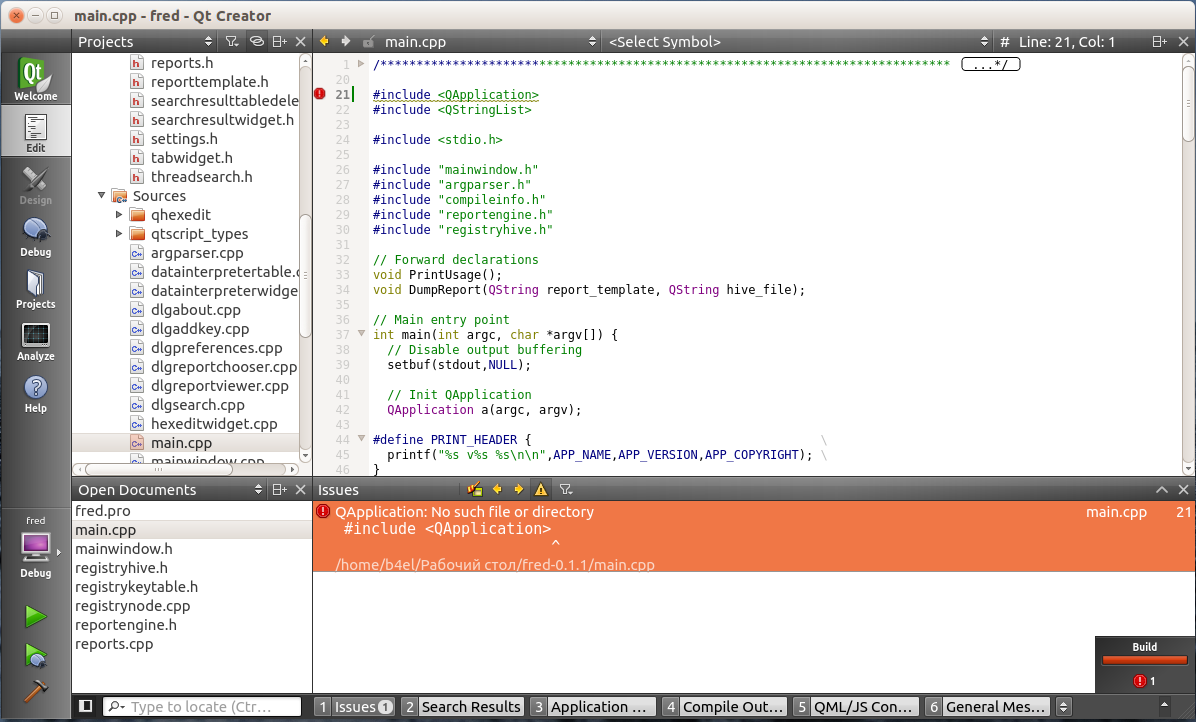
\includegraphics[width=0.8\linewidth]{bib}}
\caption{Отсутствие в Qt5 необходимых библиотек}
\label{bib:bib}
\end{figure}

Из-за сложности переноса утилиты и ограничений её использования, было принято решение о частичном заимствовании логики при написании самостоятельного плагина к системе.

\subsubsection{Этап третий --- <<разработка>>. Выбор метода получение информации из реестра}
Рассмотренные выше утилиты позволяют работать с реестром лишь через себя. Использование Cntpw как полностью, так и частично невозможно из-за ограничений лицензий. Утилита fred так же ограничена в использовании, но у него имеются открытые исходные коды в свободном доступе, а значит, на них можно опираться при разработке своей программы.

\subsubsection{Этап третий --- <<разработка>>. Разработка приложения}
Для получения данных из реестра, фактически, нужно проводить реверс формата исходных файлов реестра Windows. Первым шагом стоит определения структуры файла. Он (файл) оказался бинарным (рис.~\ref{hex:hex}).

\begin{figure}[ht!]                        % тут рисунок 5 - Представление файла DEFAULT в HEX редакторе
\center{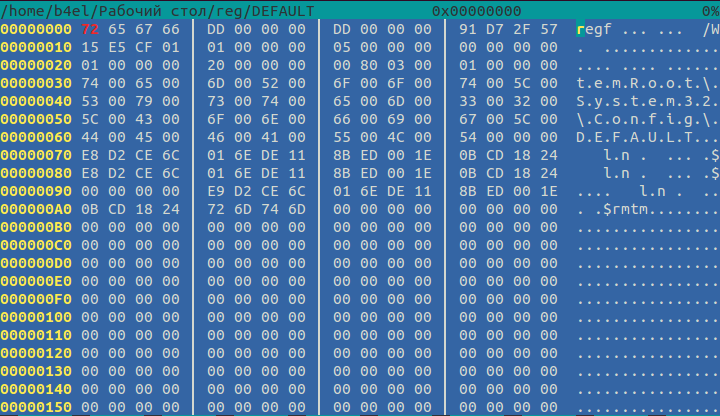
\includegraphics[width=0.8\linewidth]{hex}}
\caption{Представление файла DEFAULT в HEX редакторе}
\label{hex:hex}
\end{figure}

Для работы с бинарными файлами используется библиотека QDataStream. Пример работы первой версии программы, выводящей строковые переменные, представлен ниже (рис.~\ref{source:source}).

\begin{figure}[ht!]                        % тут рисунок 6 – Исходный код программы
\center{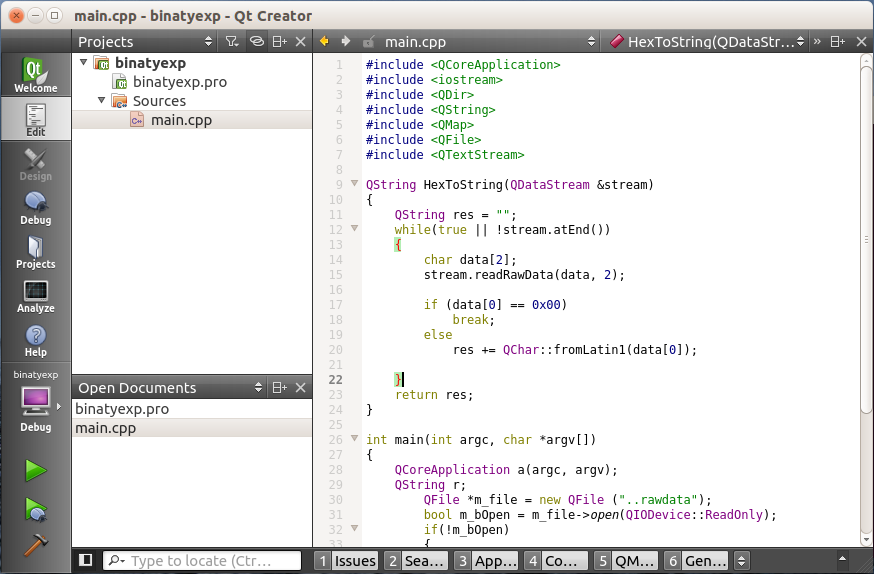
\includegraphics[width=0.8\linewidth]{source}}
\caption{Исходный код программы}
\label{source:source}
\end{figure}

Процесс извлечения строковых переменных из реестра можно увидеть на рисунке~\ref{izv:izv}.

\begin{figure}[ht!]                        % тут Рисунок 7 – Извлечение строковых переменных из реестра
\center{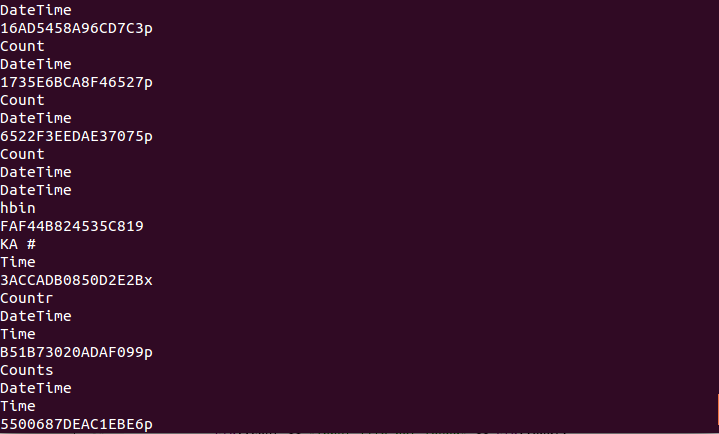
\includegraphics[width=0.7\linewidth]{izv}}
\caption{Извлечение строковых переменных из реестра}
\label{izv:izv}
\end{figure}

\subsubsection{Задачи на следующий семестр}
В ходе дальнейшей разработки планируется определить условную разметку файла, которая определяет принадлежность каждого раздела к другому, а также получить данные из разделов-листьев и перевести эти данные в xml-представление.

\subsubsection{Ссылки на Интернет-ресурсы}
Ссылки:
\begin{itemize}
  \item страница утилиты fred --- https://www.pinguin.lu/fred;
  \item пример использования cntpw --- http://habrahabr.ru/post/94764;
  \item страница утилиты chntpw --- http://pogostick.net/~pnh/ntpasswd;
  \item информация по реестру --- http://www.forensicswiki.org/wiki/Windows\_Registry;
  \item описание видов лицензий --- http://www.gnu.org/licenses/licenses.html;
  \item описание xml --- https://ru.wikipedia.org/wiki/XML.
\end{itemize}

\clearpage
